\chapter{Results}

In order to demonstrate its efficiency, the \texttt{Cavalry} renderer created in this project is compared with two of the most famous renderers used in academia:

\begin{itemize}
    \item The \texttt{pbrt} renderer, version 3. This is a comprehensively documented and optimized CPU renderer, and it is accompanied and documented by the ``PBRT'' book \cite{pharr2016physically}. At the time of writing, a 4th version of \texttt{pbrt} is under development. The 4th version will include GPU support, but due to stability issues, the beta version couldn't be used for comparison with \texttt{Cavalry}.
    
    \item The \texttt{Mitsuba} renderer. This is another well-known renderer with full GPU support. The renderer uses NVIDIA's Optix library for intersection detection, which is considered to have state-of-the-art performance.  
\end{itemize}

The \texttt{Mitsuba} and \texttt{pbrt} renderers are compared with \texttt{Cavalry}'s implementation of both the traditional path-tracing and the reinforcement learning path-tracing algorithms. Notice that, \texttt{Mitsuba} and \texttt{pbrt} also implement other variants of path-tracing (e.g., bi-directional path-tracing), but only the traditional path-tracing integrator of these renderers are used for comparison.

The scenes used to compare these renders are created by Benedikt Bitterli, and they were downloaded from \cite{resources16}. The creator defined these scenes for both \texttt{pbrt} and \texttt{Mitsuba}, with identical geometries and near identical materials. The \texttt{Cavalry} renderer created in this project parses the same input files as \texttt{pbrt}. It is thus ensured that all renderers are assigned the same task\footnote{One potential source of unfairness is that when rendering on \texttt{Mitsuba}, a rather naive random number generator is used, because the better RNGs of \texttt{Mitsuba} do not allow flexibly setting $spp$.}. All images are rendered on a Microsoft Surface Book 2 laptop, with a i7-8650U CPU and a GTX 1060 GPU.

For each scene, the renderers are asked to render images with an increasing amount of samples per pixel, starting from $4$ and doubling up to $1024$. The image with $1024$ $spp$ is used as a reference, and the other images are compared with the reference by computing the mean-squared-error (MSE) of pixel values. The MSE is plotted against the time spent on rendering on a log-log scale. Since MSE (i.e., variance) is inversely proportional to samples count (which is linear to rendering time), the log-log plots usually take the shape of a straight line with negative gradient.

A total of 4 scenes are selected. For each scene, an image rendered by \texttt{Cavalry} is shown, as well as the plot of MSE against rendering time. Notice that in the legends, \texttt{path} represents the path-racing implementation by \texttt{Cavalry}, and \texttt{rlpath} represents its reinforcement learning path-tracing implementation.

\thispagestyle{empty}
\enlargethispage{5\baselineskip}

\begin{figure}[H]
    \centering
    
    \begin{minipage}[t]{.99\textwidth}
        \centering
        \vspace{0pt}
        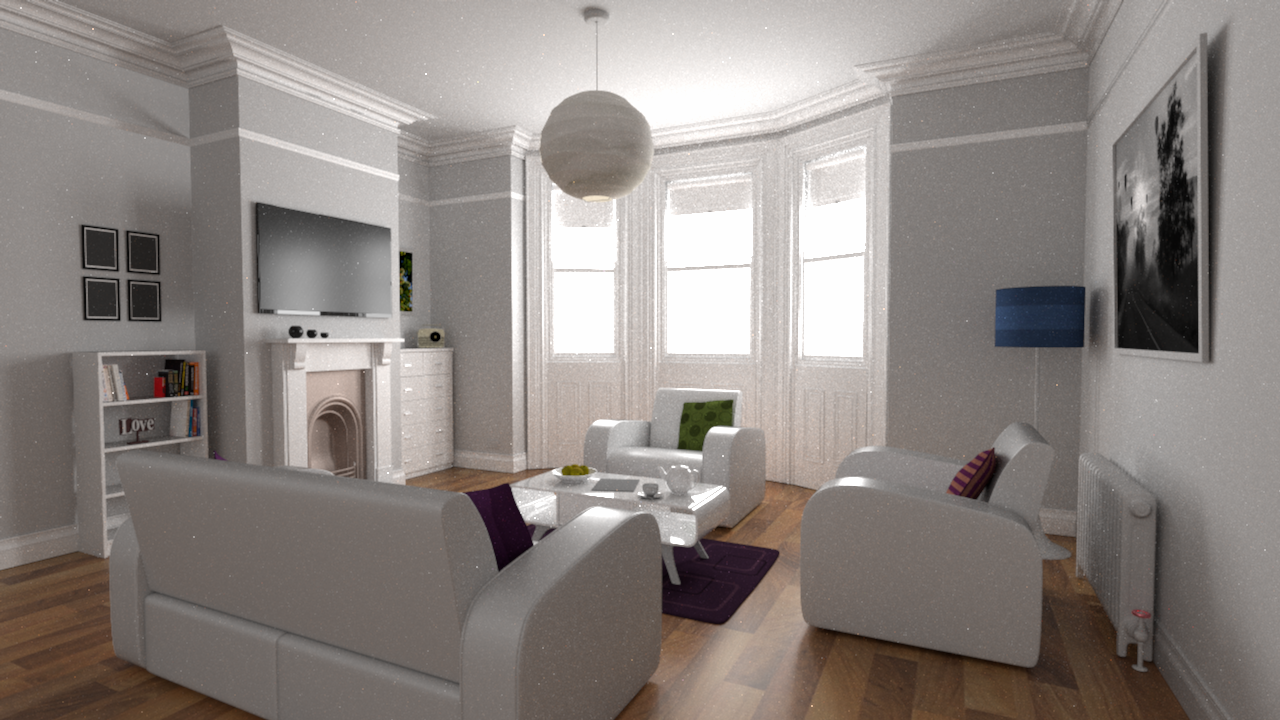
\includegraphics[width=.9\textwidth]{chapter5/living-room-2_1024spp_path.png}
    \end{minipage}
    
    \vspace{0.1cm}

    \begin{minipage}[t]{.99\textwidth}
        \centering
        \vspace{0pt}
        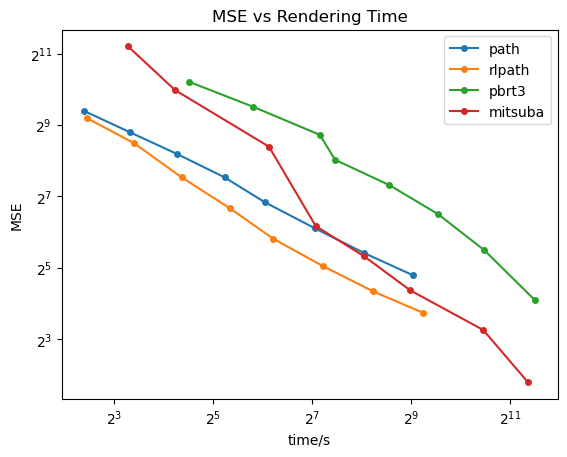
\includegraphics[width=.67\textwidth]{chapter5/error_vs_time_living_room_2.png}
    \end{minipage}
    
    \caption{The ``living-room-2'' scene.}
\end{figure}

As indicated by the plot, for this living room scene, the reinforcement learning integrator exhibits the greatest efficiency. \texttt{Mitsuba} is less efficient than \texttt{path} in the beginning, but overtakes at bigger sample counts. Naturally, all 3 GPU rendering algorithms outperform \texttt{pbrt}, which is CPU-only.

\newpage

\begin{figure}[H]
    \centering
    
    \begin{minipage}[t]{.99\textwidth}
        \centering
        \vspace{0pt}
        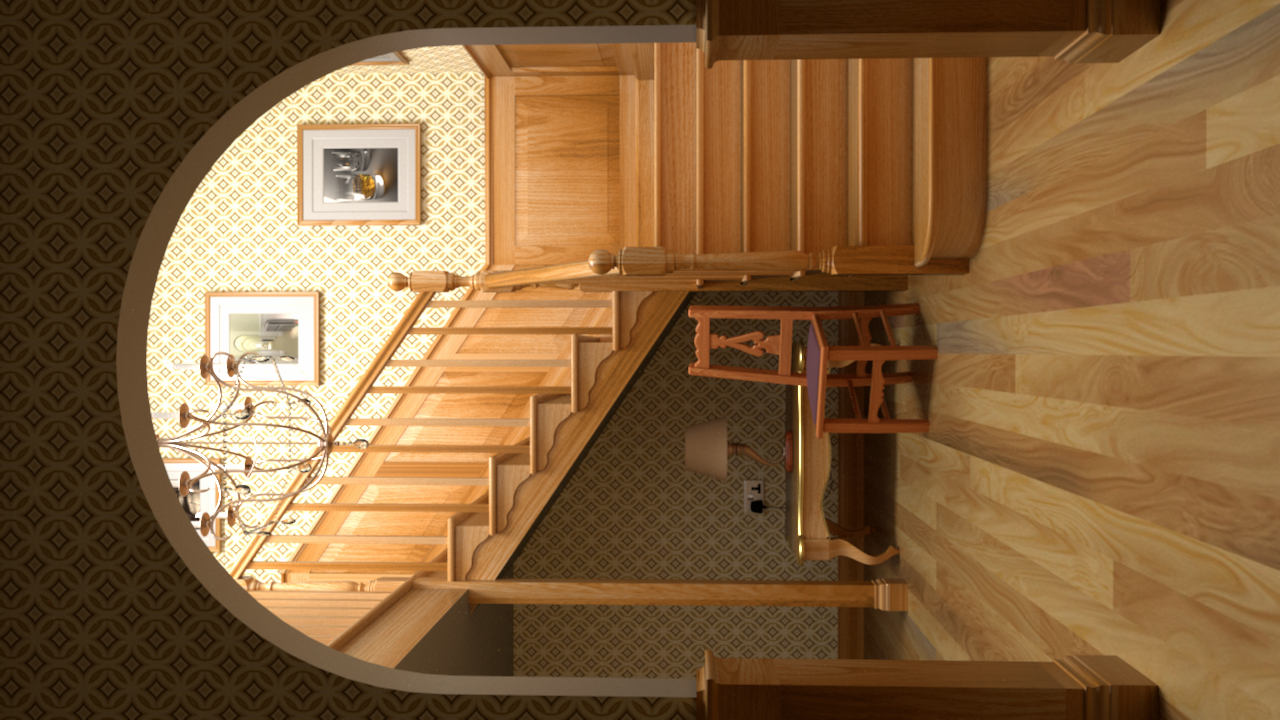
\includegraphics[width=.99\textwidth]{chapter5/staircase_1024spp_rlpath_rotated.png}
    \end{minipage}
    
    \vspace{0.3cm}

    \begin{minipage}[t]{.99\textwidth}
        \centering
        \vspace{0pt}
        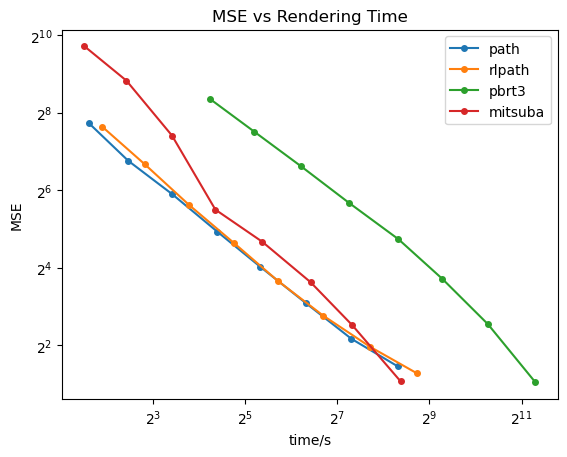
\includegraphics[width=.67\textwidth]{chapter5/error_vs_time_staircase.png}
    \end{minipage}
    
    \caption{The ``staircase'' scene (rendered image rotated by 90 degrees).}
\end{figure}

For this staircase scene, the reinforcement learning path-tracing algorithm no longer has an advantage over traditional path-tracing. This is explained by the more forgiving lighting situation, where the majority of the scene (floor, stairs, wall in the back) is dominated by direct illumination from the light source. In contrast, in the living room, the light source is dimmer and the inter-reflections between objects are more important. Nevertheless, in the staircase scene, both integrators of \texttt{Cavalry} outperform \texttt{Mitsuba} (except at 512$spp$) and \texttt{pbrt}. 

\newpage
\begin{figure}[H]
    \centering
    
    \begin{minipage}[t]{.99\textwidth}
        \centering
        \vspace{0pt}
        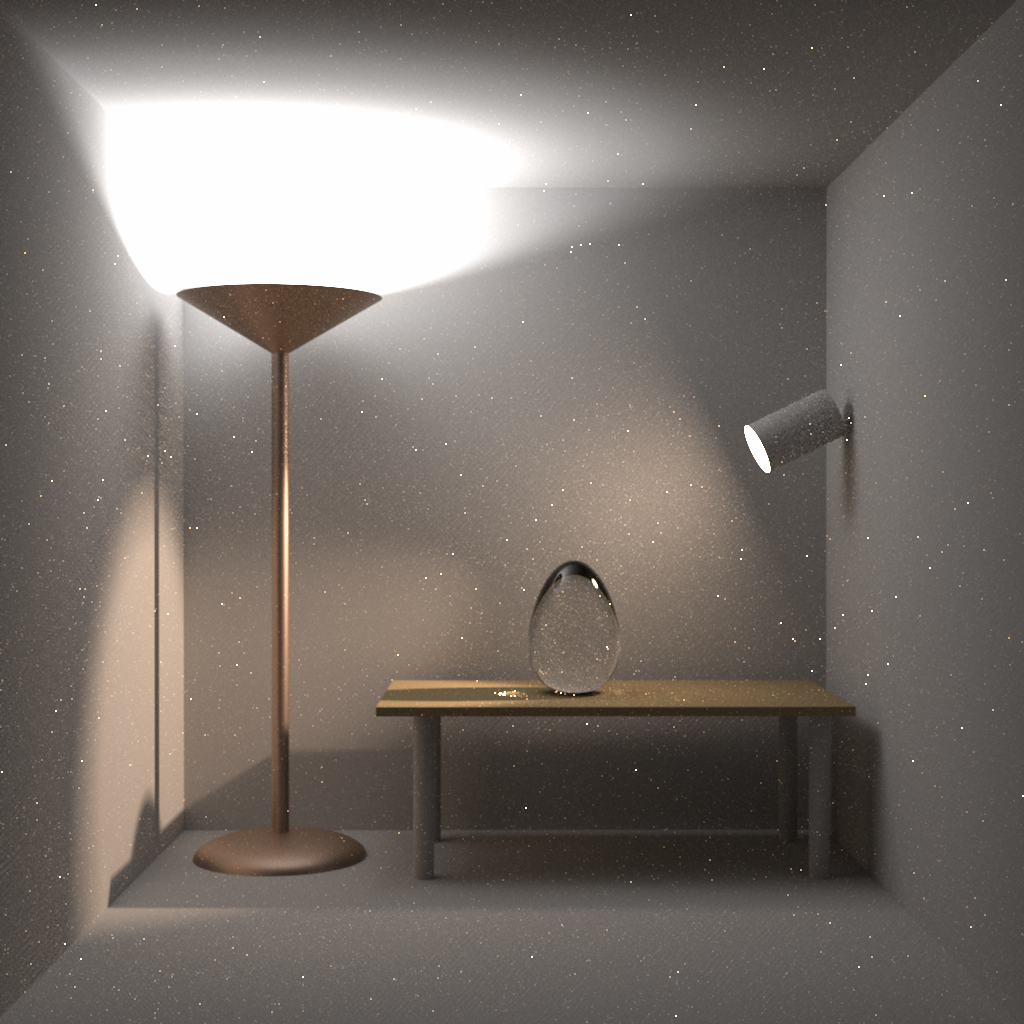
\includegraphics[width=.67\textwidth]{chapter5/veach-bidir2_1024spp_rlpath.png}
    \end{minipage}
    
    \vspace{0.3cm}

    \begin{minipage}[t]{.99\textwidth}
        \centering
        \vspace{0pt}
        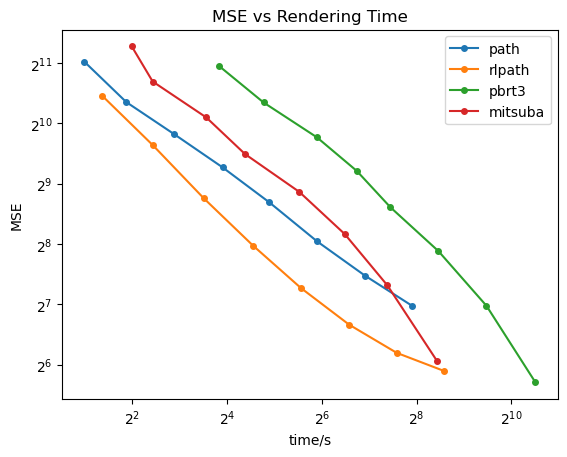
\includegraphics[width=.67\textwidth]{chapter5/error_vs_time_veach_bidir2.png}
    \end{minipage}
    
    \caption{The ``veach-bidir'' scene.}
\end{figure}

This is the scene with the difficult lighting scenario that was described in chapter \ref{chapter RL}. The advantage of \texttt{rlpath} over \texttt{path} (and the other two renderers) is the most significant here, because reinforcement learning can guide rays towards the bright region of dominant indirect illuminations.


\newpage
\begin{figure}[H]
    \centering
    
    \begin{minipage}[t]{.99\textwidth}
        \centering
        \vspace{0pt}
        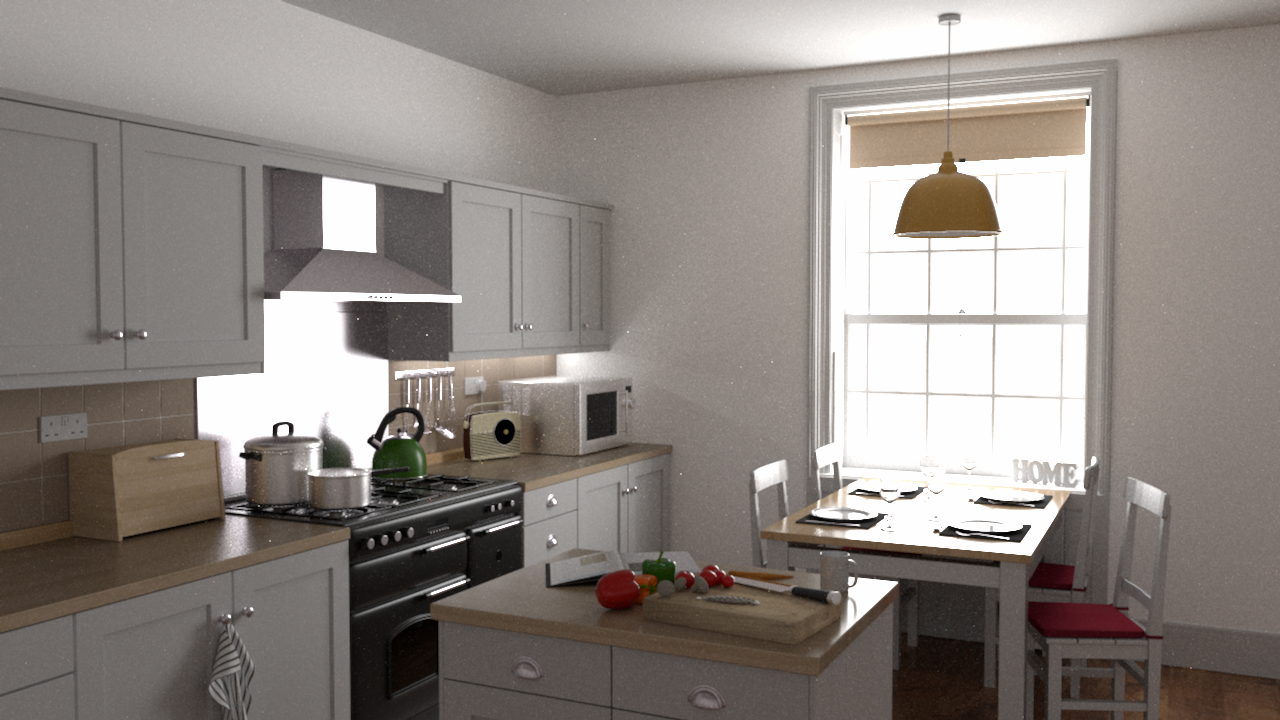
\includegraphics[width=.99\textwidth]{chapter5/kitchen_1024spp_rlpath.png}
    \end{minipage}
    
    \vspace{0.3cm}

    \begin{minipage}[t]{.99\textwidth}
        \centering
        \vspace{0pt}
        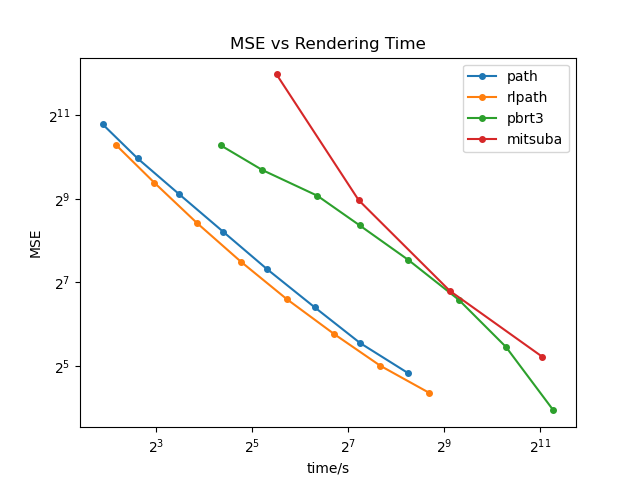
\includegraphics[width=.67\textwidth]{chapter5/error_vs_time_kitchen.png}
    \end{minipage}
    
    \caption{The ``kitchen'' scene.}
\end{figure}

In this kitchen scene, the \texttt{rlpath} integrator slightly outperforms \texttt{path}, which significantly outperforms both \texttt{pbrt} and \texttt{Mitsuba}\footnote{Peculiarly, in this scene, the \texttt{Mitsuba} GPU renderer was even outperformed by \texttt{pbrt}. It is unclear as to why this happened.}. 

\newpage

To sum up, it was found that the performance of the \texttt{Cavalry} renderer created by this project significantly outperforms the \texttt{pbrt} CPU renderer, and in many occasions, it even surpasses the \texttt{Mitsuba} GPU renderer, which uses NVIDIA's state-of-the-art intersection detection library. Moreover, it was shown that except in scenes where direct lighting dominates, the reinforcement learning path-tracing algorithm prove to be more effective than the traditional path-tracing algorithm.

%\footnote{Other parts of \texttt{Mitsuba} might not be as extremely optimized in terms of performance. For a quick but vague discussion, see \url{https://github.com/mitsuba-renderer/mitsuba2/issues/72}}